\section{Introduction}

\begin{frame}{Conventional and adaptive Therapy}
  \begin{columns}
    \begin{column}{0.45\textwidth}
      \begin{itemize}
        \item Conventional therapy @ MTD $\rightarrow$\\
        $\downarrow$ tumour burden \cite{Frei}
        \item Heterogenous sensitivity $\rightarrow$\\
        sens. $\times$ $\rightarrow$ resst. \cite{Scott}
        \item AT = $\downarrow$ , $\sim$ dose $\rightarrow$ sens. $\checkmark$ \cite{Gatenby}
        \item Drug holiday - sens. $\rightarrow\ \downarrow$ resst.
        \item AT outcome $\leftarrow$ competition
      \end{itemize}
    \end{column}
    \begin{column}{0.55\textwidth}
      \begin{figure}[h]
        \centering
        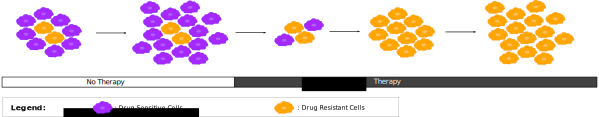
\includegraphics[width=\textwidth]{compe_release}
        \caption{Competitive release under SOC}
      \end{figure}
      \begin{figure}[h]
        \centering
        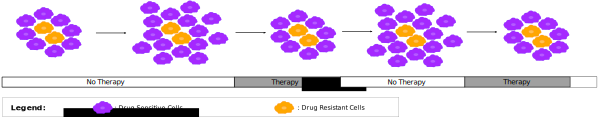
\includegraphics[width=\textwidth]{at}
        \caption{Control under AT}
      \end{figure}
    \end{column}
  \end{columns}
\end{frame}

\begin{frame}{System of study}
  \begin{itemize}
    \item Castration-Resistant Prostate Cancer (CRPC)
    \item AR pathway: prostate cells $\rightarrow$ cancer \cite{Heinlein}
    \item Therapy: ADT + Abiraterone
  \end{itemize}
  \begin{table}
    \centering
    \begin{tabular}{|l|c|c|c|c|}
    \hline
    Cell type & Test. dependent & Test. Producing & Ab. sensitive & Mechanism \\
    \hline
    $T^+$ & Yes & No & Yes & N/A \\
    $T^p$ & Yes & Yes & Yes & Cholesterol $\xrightarrow{CYP17\alpha}$ Test.\\
    $T^-$ & No & No & No & AR $\mu^n$\\
    \hline
    \end{tabular}
  \end{table}
\end{frame}

\begin{frame}{System of equations}
  \begin{columns}
    \begin{column}{0.45\textwidth}
      \begin{itemize}
        \item Logistic framework w/ dynamic carrying capacity $\approx$ env. condn.
        \item Environment = resource = $\{O_2,test\}$
        \item No $\mu^n$, no spatial structure, well mixed
        \item Defined $\mathbb{R}_{\geq 0}$, $y_i < 1 =$ extinction
      \end{itemize}
      \begin{figure}[h]
        \centering
        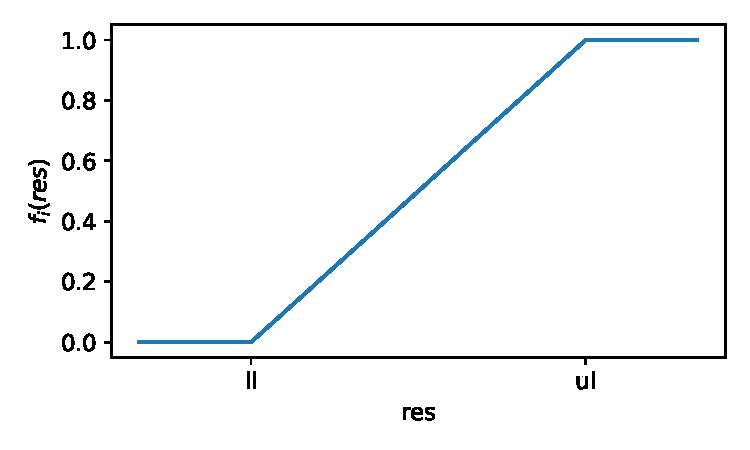
\includegraphics[width=\textwidth]{f_res}
        \caption{$f_i(res)$}
      \end{figure}
    \end{column}
    \begin{column}{0.55\textwidth}
      \begin{equation}
        \frac{dy_i}{dt} = r_i y_i (1 - \frac{\sum_j y_j}{1 + K_{i,max} f_i(O_2) f_i(test)} )- \delta_i y_i
        \label{celleq}
      \end{equation}
      \begin{equation}
        \frac{dO_2}{dt} = p_{O_2} - \sum_i \mu_{O_2,i} y_i - \lambda_{O_2} O_2
        \label{o2eq}
      \end{equation}
      \begin{equation}
        \frac{dtest}{dt} = p_{test} y_{T^p} - \sum_i \mu_{test,i} y_i - \lambda_{test} test
        \label{testeq}
      \end{equation}
      \begin{equation}
        f_i(res) = \begin{cases}
          1 &\text{if } ul_{res,i} \leq res\\
          \frac{res-ll_{res,i}}{ul_{res,i}-ll_{res,i}} &\text{if } ll_{res,i} < res < ul_{res,i}\\
          0 &\text{if } res \leq ll_{res,i}\\
        \end{cases}
        \label{freseq}
      \end{equation}
      $i \in \{T^+,T^p,T^-\}$ and $res \in \{O_2,test\}$.
    \end{column}
  \end{columns}
\end{frame}
